\chapter{Asking Millionaires How They Got Rich: Houston}

This lecture is best read as a piece of commercial mathematics. We are not led through a blackboard derivation; we are led through a sequence of operating cases, each of which contributes one part of a larger update rule. The order is important. We begin with a number large enough to provoke curiosity, then move through examples of earning, holding, losing, correcting, redeploying, and finally selling oneself as a durable economic asset. If we keep close to that order, the lecture becomes much sharper on the page than it does when flattened into generic advice.

\section{Revenue Before Theory}

The lecture opens in medias res with a restaurant owner saying that he occupies only \(4600\) square feet and did one million dollars in revenue in a single month. Only after this do we widen to Houston as one of the cities in the world with an unusually high concentration of millionaires. The pedagogical move is deliberate: first scale, then explanation.

Let us write down the teaser carefully. If \(A\) is the restaurant footprint and \(R_{\mathrm{mo}}\) the one-month revenue, then
\begin{align}
A &= 4600\ \text{sq ft},\\
R_{\mathrm{mo}} &= 1{,}000{,}000\ \text{USD}.
\end{align}
The corresponding monthly revenue density is
\begin{equation}
\rho_{\mathrm{mo}}
=
\frac{R_{\mathrm{mo}}}{A}
=
\frac{1{,}000{,}000}{4600}
\approx
217.4\ \text{USD}\,\text{sq ft}^{-1}\,\text{month}^{-1}.
\end{equation}
If one annualizes that single-month run rate, one gets
\begin{equation}
\rho_{\mathrm{yr}}^{(\mathrm{annualized\ teaser})}
=
12\,\rho_{\mathrm{mo}}
\approx
2608.7\ \text{USD}\,\text{sq ft}^{-1}\,\text{year}^{-1}.
\end{equation}

We should not overread this first move. The lecture is not yet claiming that this annualized figure is the restaurant's true year. It is merely placing a large number on the table and asking us to carry it forward as a puzzle. The rest of the chapter is an attempt to understand what sort of operator, capital discipline, and service logic can sit behind such density.

\section{Making Money and Keeping Money}

The first interview gives us a speaker in the concierge space: private jet charter, yacht charter, exotic cars, and the whole luxury-service ecosystem. The host first asks the obvious question, namely what was the most money ever made in a single year, and the answer is substantial:
\begin{equation}
Y_{\mathrm{concierge}} \in [2.5,5]\ \text{million USD/year}.
\end{equation}
But the lecture does not stop at the spectacle of the number. It immediately pivots to a harder question: what was the best financial decision ever made? The answer is severe and memorable. Learn to hold on to money.

\begin{definition}
For the purpose of these notes, we introduce a simple editorial bookkeeping language. Let \(Y_t\) denote income earned in period \(t\), \(C_t\) consumption or cash leakage, and \(L_t\) losses absorbed in that period. We then define retained capital by
\begin{equation}
K_t = Y_t - C_t - L_t,
\end{equation}
and accumulated deployable wealth by
\begin{equation}
W_{t+1}=W_t+K_t.
\end{equation}
\end{definition}

No such notation is written on screen in the lecture. It is a cautious reconstruction of the economic logic that the speaker states in plain language. Many people can generate \(Y_t\); the rare event is to preserve enough of it that \(K_t\) remains materially positive.

The interview then adds a second ingredient, though the transcript is slightly garbled in its exact wording: keep the right people around you. The sense is clear even if the line is imperfect. The luxury business depends on relationships, introductions, and proximity to people whose preferences can support large transactions. So from the first case onward, wealth is presented not as solitary arithmetic, but as arithmetic embedded in networks.

\subsection{Question \& Answer}

\paragraph{Question.} Why does high income so often fail to become wealth?

\paragraph{Answer.} Because gross earnings and retained capital are not the same object. In the lecture's language, many can make money, but far fewer can keep it. In our notation, the danger is not a small \(Y_t\); it is the collapse of \(K_t\) under consumption, leakage, or badly handled loss.

The host then pauses and recaps with visible surprise. It is the first interview of the day, and already the earnings are measured in millions. That recap should remain in the chapter. It tells us that the first case is not just biography; it is the first governing principle.

\begin{figure}
\centering
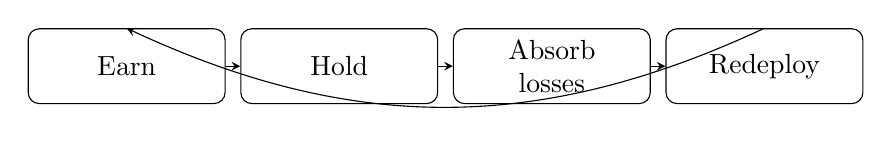
\begin{tikzpicture}[>=stealth, node distance=2.7cm, every node/.style={draw, rounded corners, minimum width=2.5cm, minimum height=0.95cm, align=center}]
\node (earn) {Earn};
\node (hold) [right of=earn] {Hold};
\node (loss) [right of=hold] {Absorb\\losses};
\node (redeploy) [right of=loss] {Redeploy};
\draw[->] (earn) -- (hold);
\draw[->] (hold) -- (loss);
\draw[->] (loss) -- (redeploy);
\draw[->, bend left=25] (redeploy.north) to (earn.north);
\end{tikzpicture}
\caption{Editorial schematic of the lecture's recurrent capital recursion. The chapter returns to this pattern in different industries: income is not the endpoint, but the beginning of a retention-and-redeployment loop.}
\end{figure}

\section{Redirection, Losses, and the First-Business Problem}

The next long interview changes the tone. We move from a speaker who always seems already to have been inside the money flow to someone whose path bends several times: computer science, then biology, then medicine, then emergency-room practice, and then business and real estate. The lecture is making a pedagogical point here. Wealth-building does not require a perfectly linear early identity. It may require that one learn from a position long enough and then move.

That biographical flexibility leads directly into an economic hardening. The host asks again about the largest single year of earnings. The answer is carefully qualified: there were years of losses, and there were good years around four to five million dollars.
\begin{equation}
Y_{\mathrm{doctor,\ good}} \in [4,5]\ \text{million USD/year}.
\end{equation}
But the speaker immediately interprets those years through the language of repair. Good years offset prior losses and then fund growth.

\paragraph{A worked capital update.} The logic unfolds in the lecture in a very definite order:
\begin{enumerate}
\item Some early periods are loss-making, so one may have \(L_t > Y_t\).
\item Later periods may produce large positive \(Y_t\).
\item Those positive years do not begin as discretionary wealth; they first repair accumulated damage.
\item Only after losses are absorbed does positive retained capital become available for new growth.
\end{enumerate}

This is where the chapter becomes more austere. The speaker says the first business is always the hardest; that it took years to make it profitable; and that there were stretches of ninety-six hours straight. The lecture is no longer content to say ``follow your passion.'' It is forcing us to think in terms of error, loss, and correction.

\subsection{Question \& Answer}

\paragraph{Question.} Why is the first business so hard?

\paragraph{Answer.} Not merely because it takes time, but because it is the first place where ego blocks learning. The speaker's rule is that one must lose the ego and take blame for everything. Even if another person made the immediate mistake, the deeper question is still local to the operator: why was that person chosen, trained, or motivated in that way?

We may summarize this correction logic by the schematic
\begin{equation}
\text{failure}
\longrightarrow
\text{self-audit}
\longrightarrow
\text{better hiring/training/motivation}
\longrightarrow
\text{corrected operation}.
\end{equation}

Once this has been said, the host asks where people should invest their money in order to grow what they have. The answer begins with a warning rather than a destination. Almost everybody will try to take advantage of the inexperienced and trusting novice. So before one becomes clever, one must learn to save. The lecture then adds a very ordinary but very important detail: delaying the first nice car until age thirty. The arithmetic here is simple, but its role in the chapter is fundamental. Capital that is spent too quickly is capital that cannot later be deployed.

A brief marine-industry interlude follows. It contributes little formal arithmetic, but it resets the register. One life, finite life, born and die, follow your dreams, do things with passion. In the notes we should preserve it as a breathing space between the doctor's loss-and-correction logic and the denser central restaurant case.

\section{The Restaurant as an Operating Model}

We now return to the teaser and ask the question that the opening forced upon us. The host goes into one of the most popular restaurants in Houston and interviews the owner. This is the chapter's densest worked example because it gives us a full stack: origin, scale, density, incentives, governance, owner presence, and premium service.

The origin itself is modest. The owner began in the dining room at sixteen and worked upward until the business became his own. The lecture is careful to place that before the large revenue claims. We are meant to understand that the spectacular number comes after deep operational immersion.

\paragraph{Anecdote.} The owner says that in December he did one million dollars in revenue in a \(4600\)-square-foot space, and that for the whole year he ended up right under \(10\) million dollars.

\paragraph{Claim.} The claim is not merely that the restaurant is busy. It is that the business is producing extraordinary revenue density.

\paragraph{Mechanism.} The mechanism is layered: the owner is present all the time, touches every table, knows the customers, aligns key employees to outcomes, keeps the partnership structure legible on paper, and refuses to let premium service collapse into a flat refusal.

Let \(R_{\mathrm{yr}}\) denote the reported full-year revenue. Then
\begin{align}
R_{\mathrm{yr}} &\approx 10{,}000{,}000\ \text{USD},\\
\rho_{\mathrm{yr}} &= \frac{R_{\mathrm{yr}}}{A}
\approx
\frac{10{,}000{,}000}{4600}
\approx
2173.9\ \text{USD}\,\text{sq ft}^{-1}\,\text{year}^{-1}.
\end{align}
This sits near, though not exactly on, the owner's spoken figure of roughly ``\(2300\) to \(2400\) a square foot.'' Since the transcript gives rounded and partly colloquial numbers, we should resist the temptation to harmonize them too aggressively. The important point is comparative: by the owner's account, almost nobody in the city does this kind of density.

\subsection{Question \& Answer}

\paragraph{Question.} How can a \(4600\)-square-foot restaurant produce this kind of revenue?

\paragraph{Answer.} The lecture answers this by accumulation of mechanisms, not by a single hidden formula. The arithmetic is only the surface. Underneath it sit owner presence, service quality, employee incentives, and pricing power.

A clean way to see the order is this:
\begin{enumerate}
\item Fix the footprint \(A=4600\ \text{sq ft}\).
\item Record the December revenue \(R_{\mathrm{mo}}=1{,}000{,}000\ \text{USD}\).
\item Compute monthly density \(\rho_{\mathrm{mo}}\approx 217.4\ \text{USD}\,\text{sq ft}^{-1}\,\text{month}^{-1}\).
\item Record the annual figure \(R_{\mathrm{yr}}\approx 10{,}000{,}000\ \text{USD}\).
\item Compute annual density \(\rho_{\mathrm{yr}}\approx 2173.9\ \text{USD}\,\text{sq ft}^{-1}\,\text{year}^{-1}\).
\item Interpret the size of the number through operating structure rather than through magic.
\end{enumerate}

The employee-alignment piece is unusually explicit. The owner tells key employees that if the business reaches a target at year end, they will receive a bonus. Formally we may write
\begin{equation}
B_i=
\begin{cases}
b_i, & \text{if the target }T\text{ is reached},\\
0, & \text{otherwise},
\end{cases}
\qquad
b_i\in\{5000,10000\}\ \text{USD}.
\end{equation}
This is not a general theory of compensation. It is a sharply legible threshold incentive.

The service model is equally explicit. When asked about never saying no, the owner explains that in the restaurant business, especially at the premium end, no one wants to hear that word. Hence the business converts extraordinary requests into extraordinary service and then charges for the transformation. If a car must be sourced from the Rolls-Royce dealer and delivered, the rule is:
\begin{equation}
P_{\mathrm{client}}=(1+m)P_{\mathrm{source}},
\qquad
m=0.20.
\end{equation}
Again the arithmetic is simple, but it matters. The refusal has been converted into fulfillment, and fulfillment into billable value.

The lecture then adds two more pieces that a weaker summary would omit. First, paperwork: if one opens a business with a partner, everything must be written out, and there must be a decision maker when disagreement occurs. Second, communication: communication is called the number one thing in a successful business. These sound administrative, even dull, beside the Ferrari and Rolls-Royce imagery, but the lecture makes them adjacent for a reason. Premium service is not possible without hard governance underneath it.

The host's recap after this interview should remain audible in the chapter. He is impressed not only by the numbers, but by the sight of an owner in the middle of a lunch rush who still knows every table and every customer. That is not empty admiration. It is the lecture's way of naming owner presence as part of the productive apparatus.

\section{Where Surplus Cash Goes}

Once the restaurant case has established that great operating businesses can throw off remarkable revenue, the lecture pivots to the next question: where does surplus cash go? The answer now comes through a cluster of shorter interviews, and we should preserve that clustering rather than compress it into a single anonymous doctrine.

We begin with a real-estate investor who also owns restaurants and a shipping-container park. The advice is concrete and local: get into areas that are beginning to gentrify, but get there early; look at where other investors are already moving; get around schools; watch for new HEBs and Amazon-centered shopping development; start buying there before the consensus arrives. The lecture is not formal here, but the structure is easy to see. One is trying to buy exposure before the development signal becomes obvious to everybody else.

The same speaker then gives a second rule, which is again more process than theory: get around people doing what you want to do, find a mentor, continue getting better, and just start. The chapter should keep that sequence. It is part of the lecture's anti-perfectionism.

The next cases widen the frame. One speaker says the central shift is to think in terms of growing one's own business rather than remaining an employee. Another, after twenty-three years of employment, now runs a propane-export business and says that relationships are the most important thing in life and in business. A later entrepreneur says that if he could begin again, he would raise capital and surround himself with really good people from day one.

By this point the lecture has built up a scale of reported outcomes:
\begin{align}
Y_{\mathrm{concierge}} &\in [2.5,5]\ \text{million USD/year},\\
Y_{\mathrm{doctor,\ good}} &\in [4,5]\ \text{million USD/year},\\
Y_{\mathrm{real\ estate\ operator}} &\approx 2\ \text{million USD/year},\\
Y_{\mathrm{medical\ sales}} &\in [0.4,0.5]\ \text{million USD/year}.
\end{align}
The point of listing these is not comparison for its own sake. It is to show that the lecture keeps circling the same structural question across different scales.

\subsection{Question \& Answer}

\paragraph{Question.} Once surplus cash exists, where should it go first, and what must remain liquid?

\paragraph{Answer.} The lecture gives an ordered heuristic rather than a theorem. Real estate is named first. But before one becomes too adventurous, one should preserve a buffer of cash measured in months of spend. Only after that does the lecture move toward broad-market exposure through the S\&P 500.

If \(S_{\mathrm{mo}}\) is monthly spend, then the recommended liquidity reserve is
\begin{equation}
B_{\mathrm{cash}} \in [6,12]\;S_{\mathrm{mo}}.
\end{equation}
Thus the capital-allocation ladder takes the form
\begin{enumerate}
\item do not spend too early on status;
\item preserve a cash buffer \(B_{\mathrm{cash}}\);
\item deploy surplus first into real estate;
\item use broad-market equity exposure, named here as the S\&P 500, beyond that.
\end{enumerate}

This same section closes with a philosophical warning that still belongs to capital allocation. Do not be a sheep. If one lane is crowded and another is open, the mere fact of the crowd should not determine the action. We should not translate that into artificial game theory. In the lecture it serves a simpler function: it warns against default imitation.

\section{Sales, Self-Investment, and the Portability of Skill}

The final stretch narrows into a group of cases that are smaller in scale but broader in portability. A medical salesperson reports earnings of roughly \(400{,}000\) to \(500{,}000\) dollars in a year and explains sales through persistence, refusal to concede, and repeated demonstrations of service. In sales, the lecture says, the person is often what is being bought.

That observation is stronger than it first sounds. It takes the restaurant owner's ``never say no'' policy and generalizes it. The customer is not purchasing a detached object alone. The customer is purchasing responsiveness, reliability, and the confidence that requests will be carried to completion.

The same speaker says that one never stops investing in oneself and never stops investing in real estate. This places personal development and external capital deployment on the same line. The operator is part of the portfolio.

The engineering interview then complicates the chapter in exactly the right way. One speaker says that for him the right move was to go to college and get an engineering degree. Yet when asked whether a college degree is necessary in general, the answer is no: it depends on the skill set. This is an important late correction. The lecture has not been building toward a single prescribed life path. It has been building toward a portable structure of judgment.

The final real-estate pair drives the point home. Sell yourself first. If they like you, they buy from you. Ask enough questions, and they in effect begin to sell themselves on what you are offering.

\subsection{Question \& Answer}

\paragraph{Question.} What is the one business skill that seems to survive across all these industries?

\paragraph{Answer.} The lecture's answer is not a product skill but a human one: the ability to sell oneself through trust, service, attention, and well-placed questions. One may be in engineering, hospitality, real estate, medicine, or sales; if one cannot make oneself credible and likable in the relevant way, opportunity does not compound.

\section{Summary}

Read in order, the lecture is much tighter than it first appears. It opens with a number, turns that number into a question, and then answers the question by layering mechanisms. First we learn that income is not wealth unless something is retained. Then we learn that the first business is hard because losses and ego interfere with correction. Then we see a restaurant case in which density, incentives, governance, and owner presence produce exceptional results. From there we move outward into real-estate heuristics, liquidity buffers, indexing, non-herd thinking, and finally the portability of salesmanship itself.

The chapter can therefore be summarized by a simple sequence. We earn. We hold. We absorb losses. We correct. We redeploy. We sell ourselves well enough to repeat the cycle. That is the commercial mathematics of this lecture, and it is why the episode feels less like a collection of street interviews than like a guided study in how income becomes durable capital.